% Relatório ENEM 2024 — Dashboard Interativo
\documentclass[a4paper,12pt]{article}

\usepackage[utf8]{inputenc}
\usepackage[T1]{fontenc}
\usepackage[brazilian]{babel}
\usepackage{graphicx}
\usepackage{booktabs}
\usepackage{xcolor}
\usepackage{hyperref}
\usepackage{geometry}
\usepackage{float}
\usepackage{caption}
\usepackage{amsmath}
\usepackage{setspace}
\graphicspath{{prints/}}

\geometry{margin=3cm}
\onehalfspacing

\hypersetup{
    colorlinks=true,
    linkcolor=blue,
    urlcolor=blue,
    citecolor=blue
}

\title{Análise dos Fatores Socioeconômicos e Demográficos\\
Associados ao Desempenho no ENEM 2024 - Tipo de Escola, Escolaridade dos Pais e Perfil dos Candidatos}
\author{Érica Alves dos Santos \and Gustavo Pimentel Carvalho Costa}
\date{2026}

\begin{document}

\maketitle
\thispagestyle{empty}
\newpage

% ----------------------------------------------------------
\section{Introdução}
% ----------------------------------------------------------

O Exame Nacional do Ensino Médio (ENEM) é a principal porta de entrada para o ensino superior no Brasil, utilizado por instituições públicas e privadas como mecanismo de seleção. Criado em 1998, o exame avalia o desempenho dos estudantes em cinco áreas do conhecimento: Ciências da Natureza, Ciências Humanas, Linguagens e Códigos, Matemática e Redação.

O Brasil apresenta profundas desigualdades educacionais e socioeconômicas que se refletem nos resultados do ENEM. Estudantes de escolas privadas, com maior acesso a recursos educacionais, tendem a obter desempenho superior àqueles de escolas públicas. Da mesma forma, a escolaridade dos pais — que influencia o capital cultural e o suporte educacional disponível em casa — é um fator fortemente associado ao desempenho no exame.

Este trabalho tem como objetivo analisar o perfil dos candidatos do ENEM 2024 e investigar a relação entre fatores socioeconômicos (tipo de escola e escolaridade dos pais) e o desempenho nas cinco áreas do conhecimento. A análise é conduzida por meio de um dashboard interativo desenvolvido com Streamlit e Plotly Express.

O relatório está estruturado em quatro seções: (i) esta introdução; (ii) a metodologia e descrição da base de dados; (iii) os resultados organizados pelas duas questões de pesquisa; e (iv) a discussão dos achados, limitações e trabalhos futuros.

% ----------------------------------------------------------
\section{Metodologia e Descrição da Base de Dados}
% ----------------------------------------------------------

\subsection{Fonte dos Dados}

Os microdados do ENEM 2024 foram obtidos junto ao INEP (Instituto Nacional de Estudos e Pesquisas Educacionais Anísio Teixeira), disponibilizados publicamente no portal de dados abertos do governo federal.

\subsection{Coleta e Estrutura Original}

O conjunto bruto é composto por três arquivos CSV:

\begin{itemize}
    \item \textbf{PARTICIPANTES\_2024.csv}: 4.332.944 registros com dados demográficos e respostas ao questionário socioeconômico (38 colunas).
    \item \textbf{RESULTADOS\_2024.csv}: 4.332.944 registros com as notas, presença e informações escolares (42 colunas).
    \item \textbf{ITENS\_PROVA\_2024.csv}: 5.550 registros com metadados dos itens das provas.
\end{itemize}

Após a junção dos arquivos de participantes e resultados (merge por índice, uma vez que ambos possuem o mesmo número de linhas e não compartilham uma chave explícita), partiu-se de aproximadamente 4,33 milhões de inscrições.

\subsection{Critérios de Filtragem}

Foram aplicados os seguintes filtros, nesta ordem:

\begin{enumerate}
    \item \textbf{Remoção de treineiros} (IN\_TREINEIRO = 1): candidatos que realizaram a prova como treino, sem interesse em vagas, foram excluídos pois não representam o perfil típico de ingresso no ensino superior.
    \item \textbf{Remoção de ausentes}: mantidos apenas candidatos presentes em todas as quatro provas objetivas (CN, CH, LC, MT). Ausentes em qualquer prova distorcem as análises comparativas.
    \item \textbf{Remoção de candidatos sem informação de escola}: excluídos registros sem tipo de dependência administrativa da escola.
    \item \textbf{Remoção de notas ausentes}: linhas com valores nulos em qualquer uma das cinco notas foram descartadas.
\end{enumerate}

\subsection{Volume Final}

Após a filtragem, restaram \textbf{960.614 candidatos}, sendo 79,4\% de escolas públicas e 20,6\% de escolas privadas.

\subsection{Variáveis Selecionadas}

No total, foram selecionadas 17 variáveis originais mais 5 colunas derivadas, conforme descrito na Tabela~\ref{tab:variaveis}.

\begin{table}[H]
\centering
\caption{Variáveis selecionadas para análise}
\label{tab:variaveis}
\begin{tabular}{ll}
\toprule
\textbf{Variável} & \textbf{Descrição} \\
\midrule
TP\_SEXO & Sexo do candidato (M/F) \\
TP\_FAIXA\_ETARIA & Faixa etária codificada (1--20) \\
TP\_COR\_RACA & Raça/cor autodeclarada \\
TP\_DEPENDENCIA\_ADM\_ESC & Dependência administrativa da escola \\
SG\_UF\_PROVA & Sigla da UF de realização da prova \\
IN\_TREINEIRO & Indicador de treineiro \\
TP\_PRESENCA\_CN/CH/LC/MT & Presença em cada prova \\
NU\_NOTA\_CN/CH/LC/MT & Notas das provas objetivas (0--1000) \\
NU\_NOTA\_REDACAO & Nota da redação (0--1000) \\
Q001--Q002 & Escolaridade do pai e da mãe (8 níveis: Nunca estudou até Pós-graduação) \\
\bottomrule
\end{tabular}
\end{table}

Colunas derivadas:
\begin{itemize}
    \item \textbf{Tipo de Escola}: Pública (Federal/Estadual/Municipal) ou Privada
    \item \textbf{Sexo, Raça/Cor, Faixa Etária, Escolaridade dos Pais}: labels legíveis
    \item \textbf{Região}: agrupamento das UFs em 5 regiões
    \item \textbf{Nota Média}: média aritmética das 5 notas
    \item \textbf{Acima de 600}: flag indicando nota $>$ 600 em pelo menos uma área
\end{itemize}

\subsection{Ferramenta de BI}

O dashboard foi desenvolvido em Python 3.10+ utilizando:
\begin{itemize}
    \item \textbf{pandas} e \textbf{numpy} para processamento dos dados
    \item \textbf{Streamlit} para a interface web interativa
    \item \textbf{Plotly Express} para visualização de dados
\end{itemize}

\subsection{Medida de Tendência Central}

Adotou-se a \textbf{mediana} como medida de tendência central em substituição à média. A escolha justifica-se pela distribuição assimétrica típica das notas do ENEM, onde a média é influenciada por valores extremos (notas muito baixas ou muito altas). A mediana, por ser robusta a outliers, oferece uma representação mais fiel do desempenho típico dos candidatos.

\subsection{Gráficos de Caracterização (G1--G8)}

Os gráficos abaixo caracterizam o perfil dos 960.614 candidatos analisados.

\subsubsection{G1 -- Distribuição por Tipo de Escola}

A Figura~\ref{fig:g1} mostra que 79,4\% dos candidatos são de escolas públicas e 20,6\% de escolas privadas.

\begin{figure}[H]
    \centering
    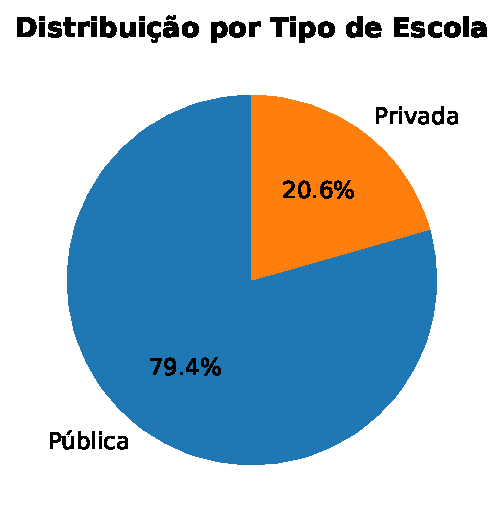
\includegraphics[width=0.6\textwidth]{g1}
    \caption{Distribuição dos candidatos por tipo de escola (G1)}
    \label{fig:g1}
\end{figure}

\subsubsection{G2 -- Distribuição por Raça/Cor}

A maior parte dos candidatos declara-se parda ou branca, conforme a Figura~\ref{fig:g2}.

\begin{figure}[H]
    \centering
    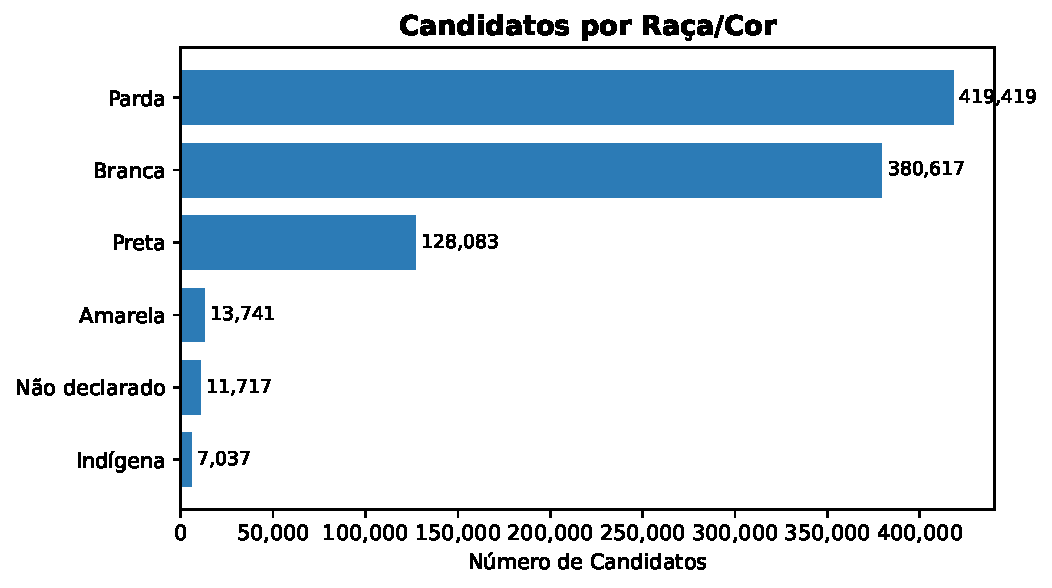
\includegraphics[width=0.8\textwidth]{g2}
    \caption{Distribuição dos candidatos por raça/cor (G2)}
    \label{fig:g2}
\end{figure}

\subsubsection{G3 -- Distribuição por Faixa Etária}

A Figura~\ref{fig:g3} apresenta a concentração de candidatos na faixa dos 17 aos 25 anos.

\begin{figure}[H]
    \centering
    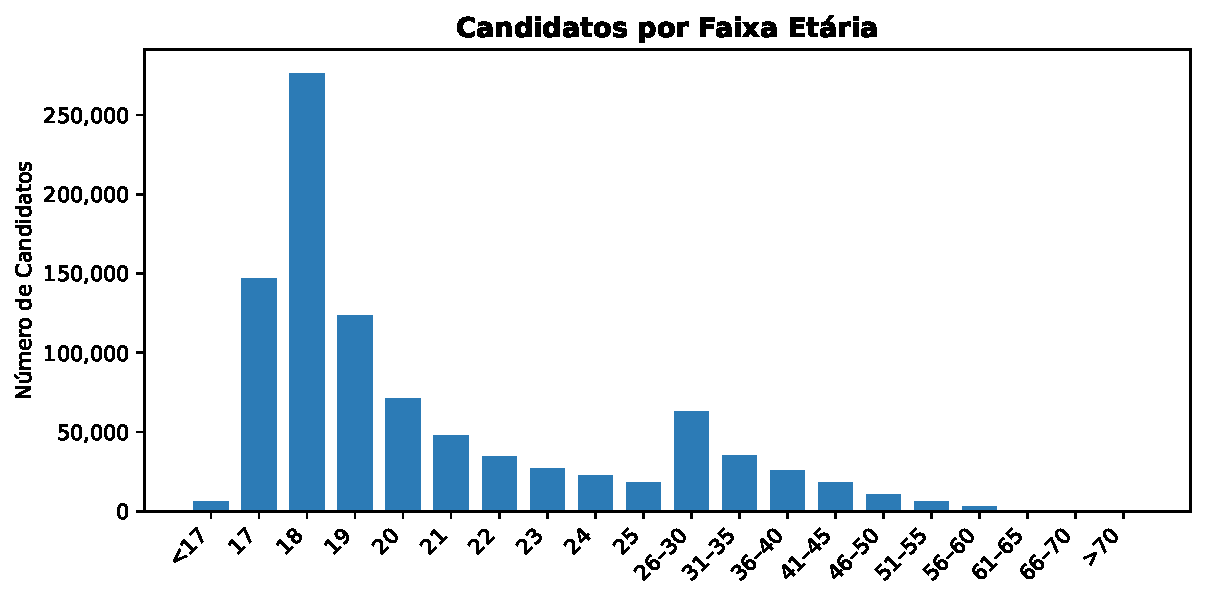
\includegraphics[width=0.85\textwidth]{g3}
    \caption{Distribuição por faixa etária (G3)}
    \label{fig:g3}
\end{figure}

\subsubsection{G4 -- Distribuição por Sexo}

A Figura~\ref{fig:g4} mostra a proporção entre candidatos masculinos e femininos.

\begin{figure}[H]
    \centering
    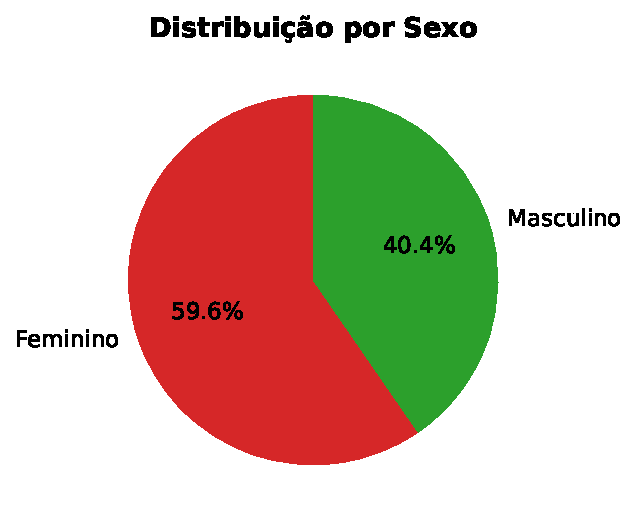
\includegraphics[width=0.55\textwidth]{g4}
    \caption{Distribuição por sexo (G4)}
    \label{fig:g4}
\end{figure}

\subsubsection{G5 -- Candidatos por Região e Tipo de Escola}

A Figura~\ref{fig:g5} segmenta os candidatos por região geográfica e tipo de escola.

\begin{figure}[H]
    \centering
    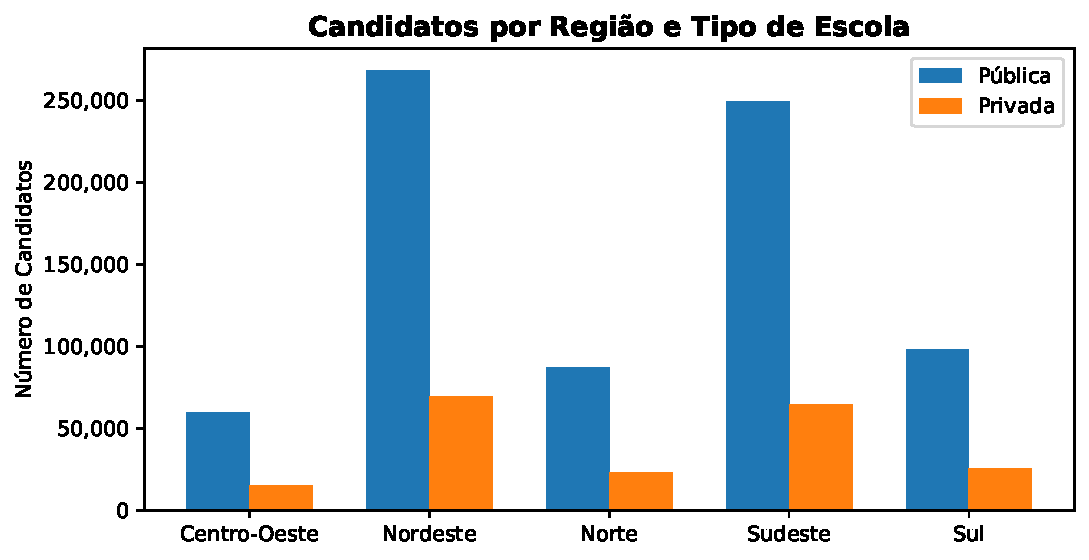
\includegraphics[width=0.85\textwidth]{g5}
    \caption{Candidatos por região e tipo de escola (G5)}
    \label{fig:g5}
\end{figure}

\subsubsection{G6 -- Candidatos por Estado}

A Figura~\ref{fig:g6} lista os estados com maior número de candidatos.

\begin{figure}[H]
    \centering
    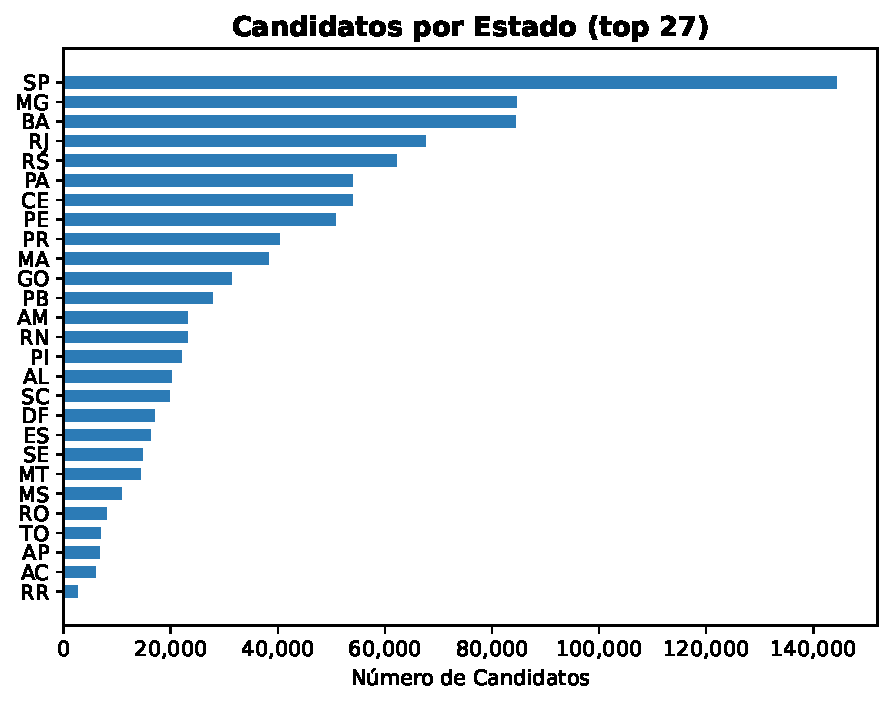
\includegraphics[width=0.8\textwidth]{g6}
    \caption{Candidatos por estado (G6)}
    \label{fig:g6}
\end{figure}

\subsubsection{G7 -- Distribuição das Notas por Área}

A Figura~\ref{fig:g7} apresenta a distribuição das notas em cada área, evidenciando a assimetria típica dos dados.

\begin{figure}[H]
    \centering
    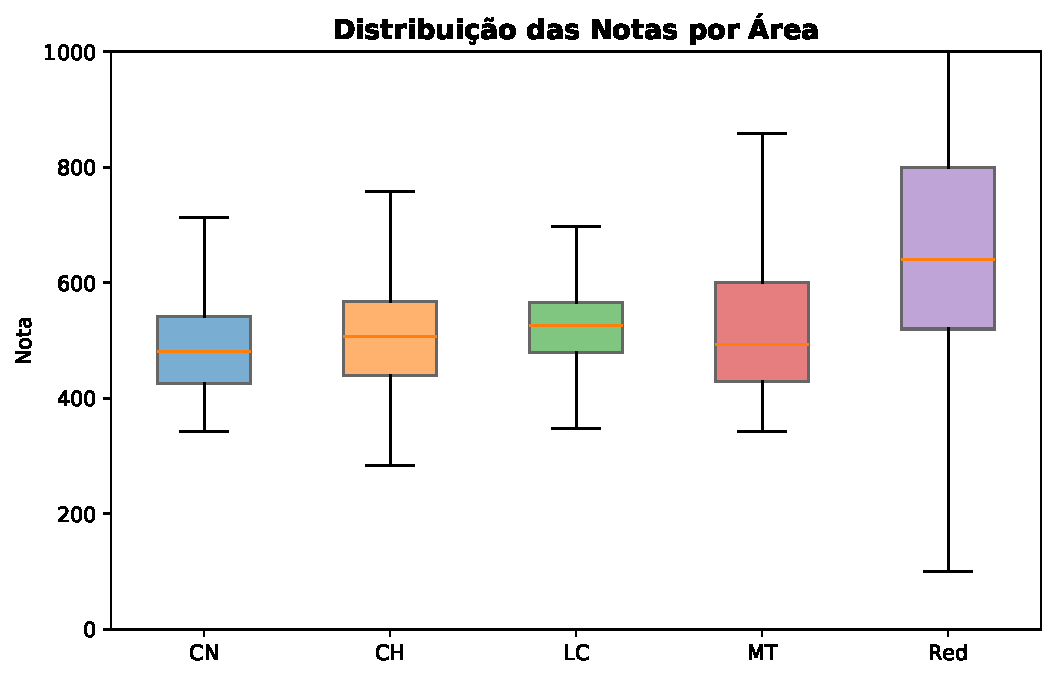
\includegraphics[width=0.85\textwidth]{g7}
    \caption{Distribuição das notas por área (G7)}
    \label{fig:g7}
\end{figure}

\subsubsection{G8 -- Mediana por Área e Tipo de Escola}

A Figura~\ref{fig:g8} compara as medianas entre escolas públicas e privadas.

\begin{figure}[H]
    \centering
    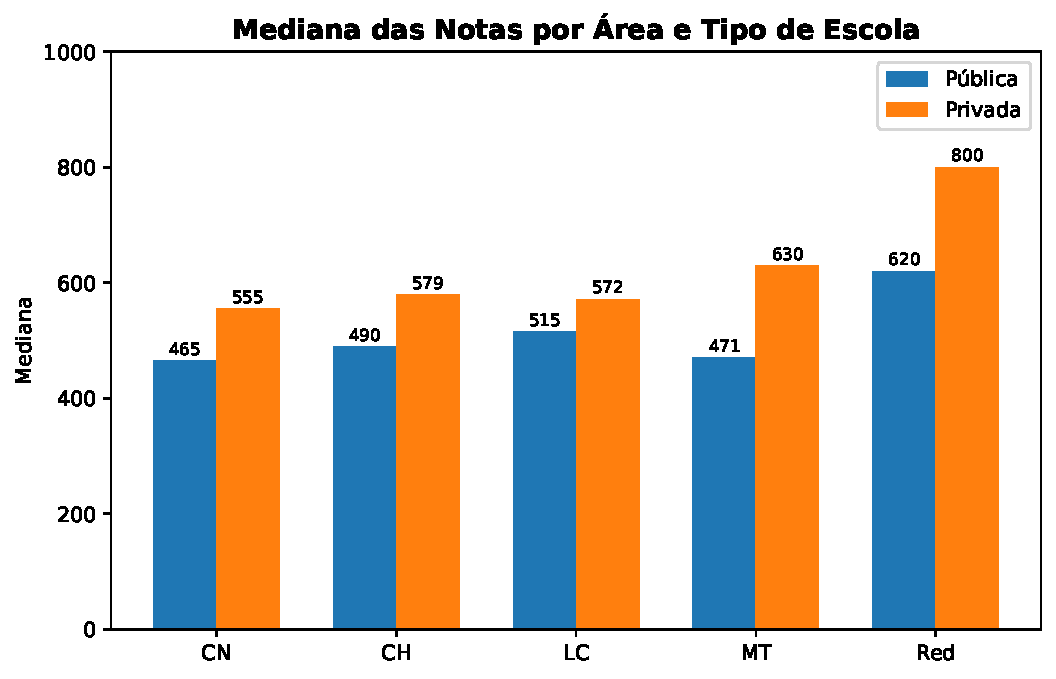
\includegraphics[width=0.85\textwidth]{g8}
    \caption{Mediana por área e tipo de escola (G8)}
    \label{fig:g8}
\end{figure}

% ----------------------------------------------------------
\section{Resultados}
% ----------------------------------------------------------

\subsection{RQ1 -- Tipo de Escola e Desempenho}

\textbf{Pergunta:} Como o tipo de escola (pública vs. privada) influencia o desempenho dos candidatos no ENEM 2024?

\subsubsection{R1.1 -- Mediana por Área: Pública vs. Privada}

A Figura~\ref{fig:r11} apresenta a mediana das notas em cada área. Candidatos de escolas privadas obtêm mediana superior em todas as áreas. A Tabela~\ref{tab:medianas} resume os valores.

\begin{table}[H]
\centering
\caption{Mediana das notas por área e tipo de escola}
\label{tab:medianas}
\begin{tabular}{lccc}
\toprule
\textbf{Área} & \textbf{Pública} & \textbf{Privada} & \textbf{Diferença} \\
\midrule
Ciências da Natureza & 464,7 & 555,4 & 90,7 \\
Ciências Humanas     & 489,8 & 579,2 & 89,4 \\
Linguagens           & 515,2 & 571,5 & 56,3 \\
Matemática           & 470,8 & 630,0 & 159,2 \\
Redação              & 620,0 & 800,0 & 180,0 \\
\bottomrule
\end{tabular}
\end{table}

\begin{figure}[H]
    \centering
    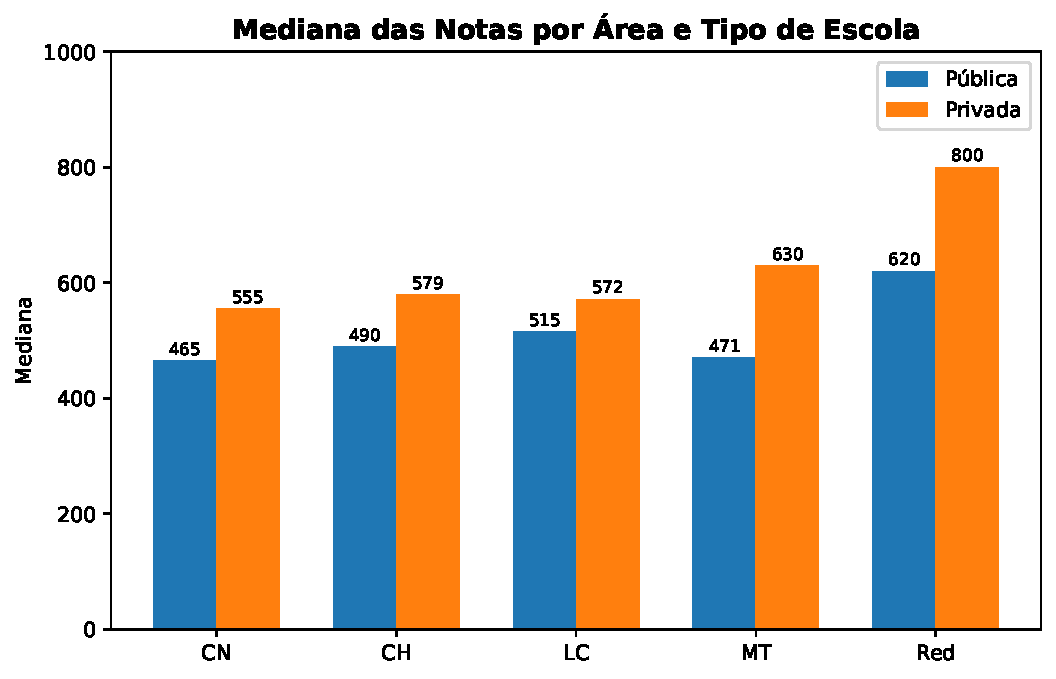
\includegraphics[width=0.85\textwidth]{g8}
    \caption{Mediana por área: pública vs. privada (R1.1)}
    \label{fig:r11}
\end{figure}

\subsubsection{R1.2 -- Distribuição das Notas: Pública vs. Privada}

A Figura~\ref{fig:g7} (seção anterior) já apresenta a distribuição geral das notas. A Tabela~\ref{tab:medianas} complementa com a comparação direta entre públicas e privadas.

\subsubsection{R1.3 -- Percentual de Candidatos com Nota Acima de 600}

A Tabela~\ref{tab:acima600} mostra o percentual de candidatos com nota superior a 600.

\begin{table}[H]
\centering
\caption{Percentual de candidatos com nota $>$ 600 por área e tipo de escola}
\label{tab:acima600}
\begin{tabular}{lccc}
\toprule
\textbf{Área} & \textbf{Pública} & \textbf{Privada} & \textbf{Diferença (p.p.)} \\
\midrule
Ciências da Natureza & 3,2\%  & 26,6\% & 23,4 \\
Ciências Humanas     & 7,6\%  & 38,6\% & 31,0 \\
Linguagens           & 5,2\%  & 28,1\% & 22,9 \\
Matemática           & 16,3\% & 58,7\% & 42,4 \\
Redação              & 50,6\% & 85,8\% & 35,2 \\
\bottomrule
\end{tabular}
\end{table}

\begin{figure}[H]
    \centering
    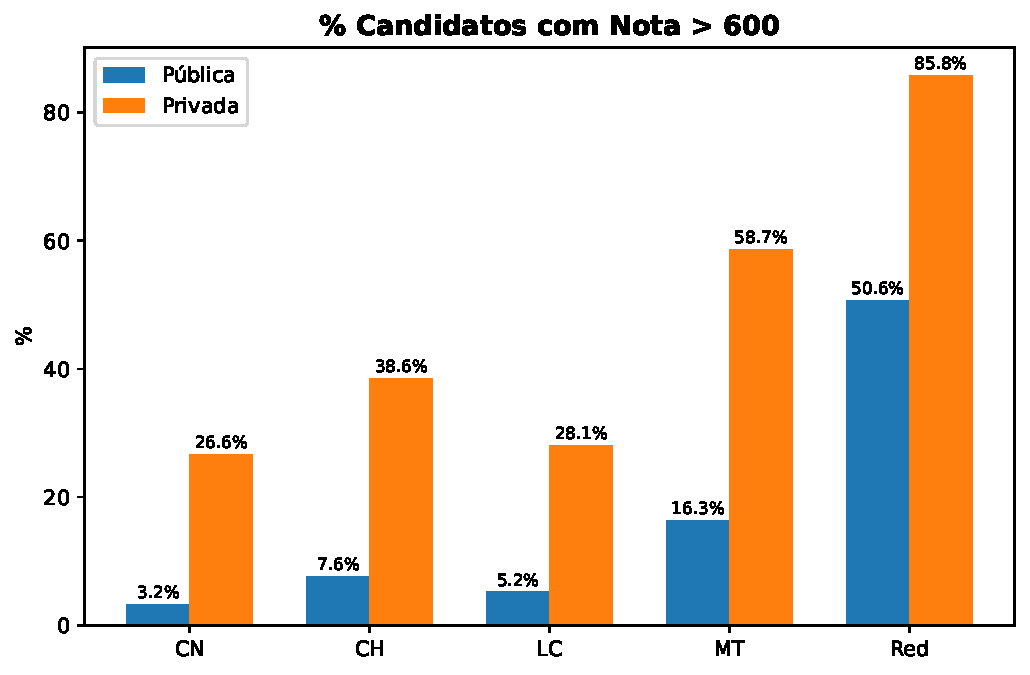
\includegraphics[width=0.85\textwidth]{r13}
    \caption{\% de candidatos com nota $>$ 600 (R1.3)}
    \label{fig:r13}
\end{figure}

\subsubsection{R1.4 -- Distribuição da Nota Média Geral}

O histograma sobreposto (Figura~\ref{fig:r14}) compara a distribuição da nota média geral.

\begin{figure}[H]
    \centering
    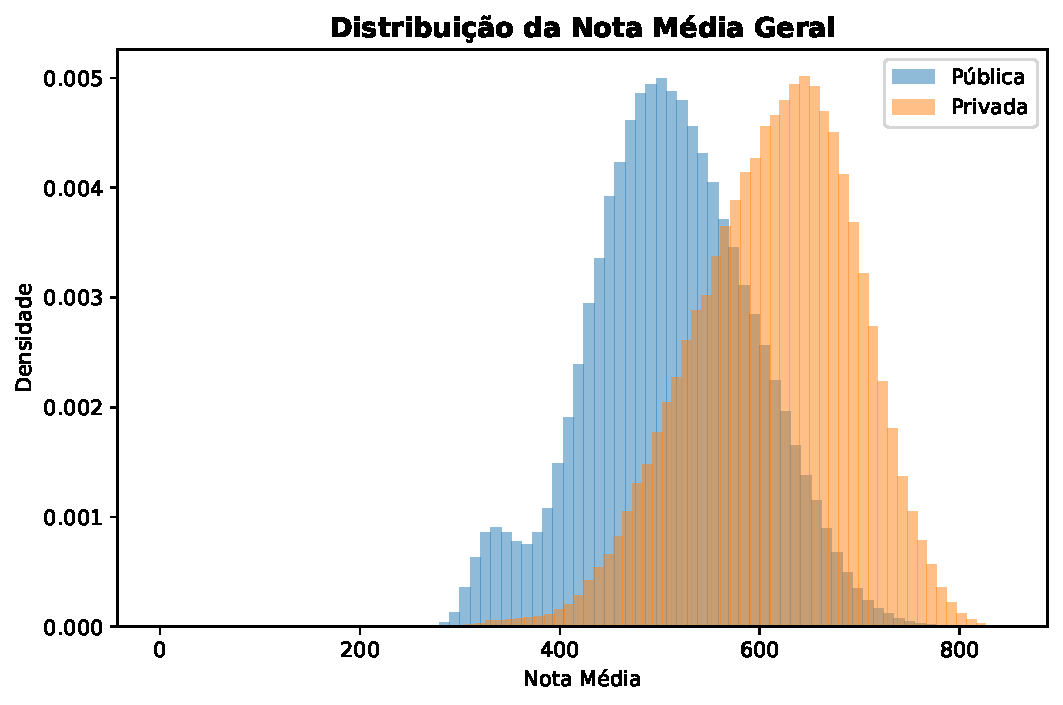
\includegraphics[width=0.85\textwidth]{r14}
    \caption{Distribuição da nota média geral (R1.4)}
    \label{fig:r14}
\end{figure}

\textbf{Achados:}
\begin{itemize}
    \item A maior diferença absoluta está em \textbf{Redação}, com 180,0 pontos de diferença na mediana.
    \item A menor diferença está em \textbf{Linguagens}, com 56,3 pontos.
    \item Em Matemática, a mediana de escolas privadas (630,0) supera a das públicas (470,8) em 159,2 pontos.
    \item A diferença é consistente em todas as áreas, porém mais acentuada em Redação e Matemática.
    \item Apenas 16,3\% dos candidatos de escolas públicas atingem nota acima de 600 em Matemática, contra 58,7\% das privadas.
\end{itemize}

\subsection{RQ2 -- Escolaridade dos Pais e Desempenho}

\textbf{Pergunta:} Qual a relação entre a escolaridade dos pais e o desempenho médio no ENEM 2024?

Os microdados do ENEM 2024 incluem as variáveis Q001 (escolaridade do pai) e Q002 (escolaridade da mãe), com oito categorias cada: \textbf{Nunca estudou}, \textbf{Fundamental incompleto}, \textbf{Fundamental completo}, \textbf{Médio incompleto}, \textbf{Médio completo}, \textbf{Superior incompleto}, \textbf{Superior completo} e \textbf{Pós-graduação}.

\subsubsection{R2.1 -- Nota Média Mediana por Escolaridade dos Pais}

A Figura~\ref{fig:r21} apresenta a mediana da nota média em função da escolaridade do pai e da mãe. Observa-se uma clara tendência ascendente: quanto maior a escolaridade dos pais, maior o desempenho médio dos candidatos.

\begin{figure}[H]
    \centering
    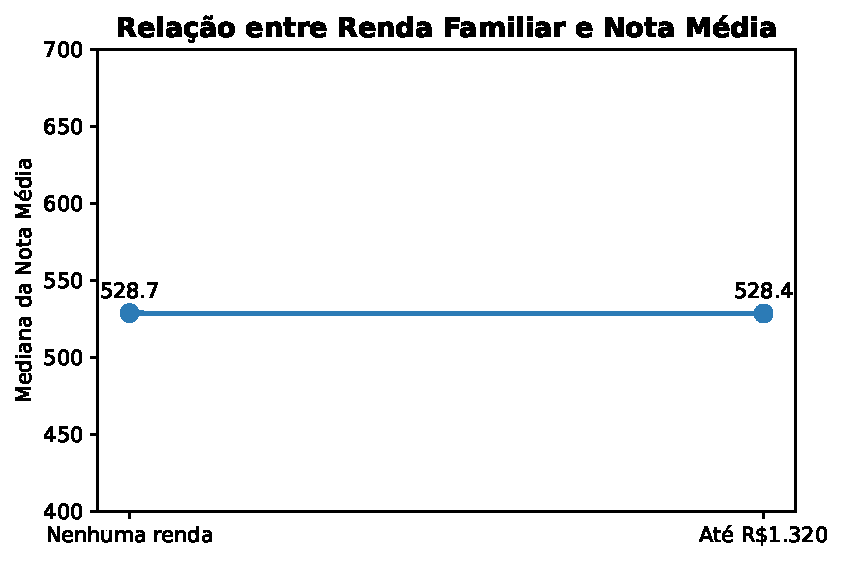
\includegraphics[width=0.8\textwidth]{r21}
    \caption{Nota média mediana por escolaridade dos pais (R2.1)}
    \label{fig:r21}
\end{figure}

\subsubsection{R2.2 -- Mediana por Área e Escolaridade do Pai}

A Figura~\ref{fig:r22} desagrega a mediana das notas por área de conhecimento e escolaridade do pai. O padrão de crescimento é consistente em todas as áreas, com destaque para Matemática e Redação, que apresentam maior amplitude entre os extremos.

\begin{figure}[H]
    \centering
    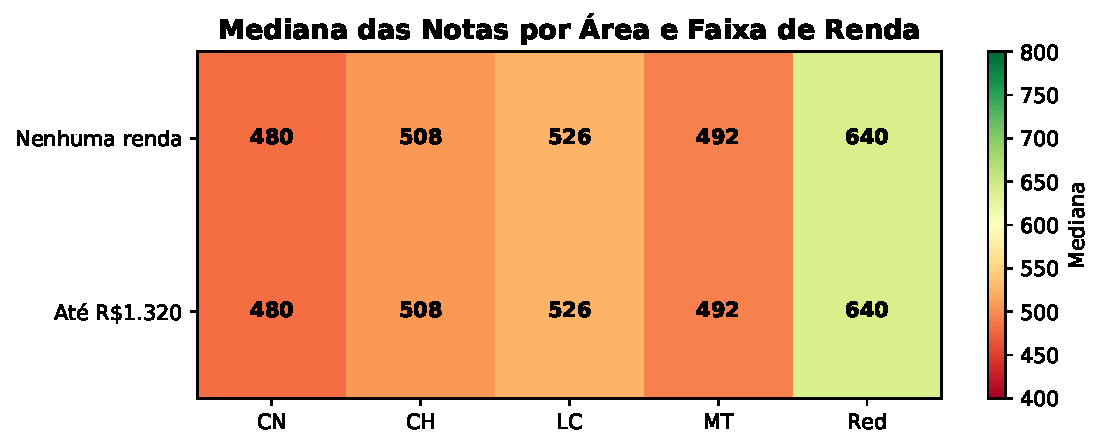
\includegraphics[width=0.9\textwidth]{r22}
    \caption{Mediana por área e escolaridade do pai (R2.2)}
    \label{fig:r22}
\end{figure}

\subsubsection{R2.3 -- Mediana por Área e Escolaridade da Mãe}

A Figura~\ref{fig:r23} mostra o mesmo recorte para a escolaridade da mãe. O padrão é semelhante ao paterno, indicando que a escolaridade de ambos os pais impacta positivamente o desempenho.

\begin{figure}[H]
    \centering
    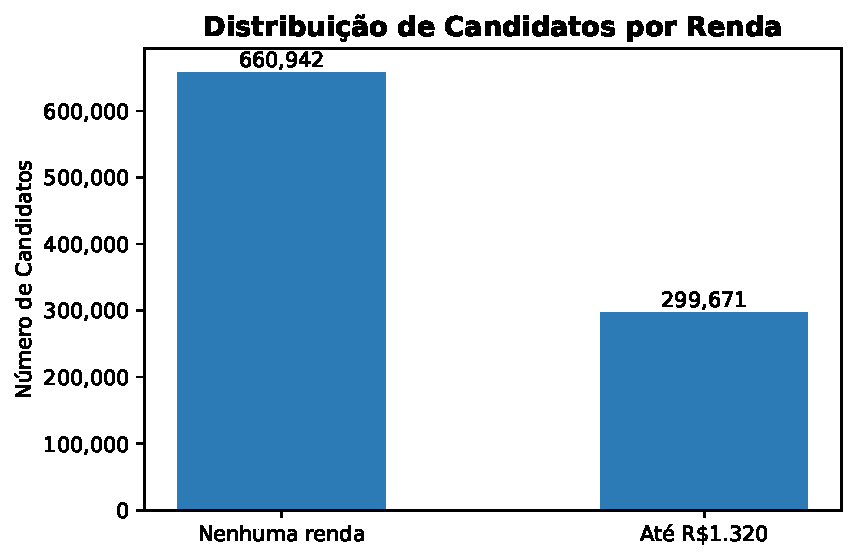
\includegraphics[width=0.9\textwidth]{r23}
    \caption{Mediana por área e escolaridade da mãe (R2.3)}
    \label{fig:r23}
\end{figure}

\subsubsection{R2.4 -- Escolaridade do Pai vs. Mãe e Nota Média}

A Figura~\ref{fig:r24} cruza a escolaridade do pai e da mãe em um heatmap, com a mediana da nota média como intensidade. A diagonal sugere que a combinação de pais com alta escolaridade produz os melhores resultados.

\begin{figure}[H]
    \centering
    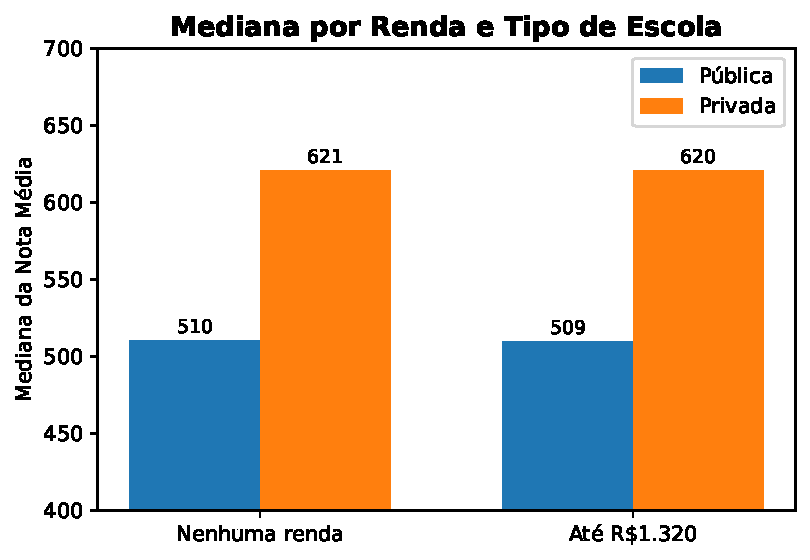
\includegraphics[width=0.8\textwidth]{r24}
    \caption{Heatmap: escolaridade do pai vs. mãe e nota média (R2.4)}
    \label{fig:r24}
\end{figure}

\textbf{Achados:}
\begin{itemize}
    \item Candidatos cujos pais têm pós-graduação apresentam mediana de nota média muito superior aos com pais que nunca estudaram, com diferença superior a 100 pontos tanto para o pai quanto para a mãe.
    \item O efeito é monotônico: a cada aumento no nível de escolaridade dos pais, a nota média mediana se eleva.
    \item A escolaridade da mãe mostra associação ligeiramente mais forte que a do pai nos níveis mais altos.
    \item O padrão se mantém em todas as áreas de conhecimento, sendo mais acentuado em Matemática e Redação.
\end{itemize}

% ----------------------------------------------------------
\section{Discussão}
% ----------------------------------------------------------

\subsection{Síntese dos Achados}

Os dados revelam que o tipo de escola é fortemente associado ao desempenho no ENEM 2024, com diferenças expressivas em todas as áreas do conhecimento. A escolaridade dos pais também apresenta forte associação com o desempenho, com efeito monotônico e consistente entre as áreas — quanto maior a escolaridade, maior a nota.

A diferença mais acentuada ocorre em Redação (180 pontos de mediana) e Matemática (159 pontos), áreas tradicionalmente associadas a maior desigualdade educacional. Linguagens apresenta o menor gap (56 pontos), possivelmente por ser uma área mais dependente de habilidades transversais.

\subsection{Relação entre RQ1 e RQ2}

A análise conjunta revela que tanto o tipo de escola (RQ1) quanto a escolaridade dos pais (RQ2) estão fortemente associados ao desempenho. Embora as variáveis estejam correlacionadas — pais com maior escolaridade tendem a matricular seus filhos em escolas privadas —, o efeito da escola se mantém significativo mesmo quando controlado indiretamente pela escolaridade parental, indicando que a qualidade do ensino ofertado é um fator determinante.

\subsection{Limitações}

\begin{itemize}
    \item \textbf{Viés de seleção}: a análise considera apenas candidatos presentes em todas as provas, excluindo ausentes que podem ter perfil sistematicamente diferente.
    \item \textbf{Dados autodeclarados}: variáveis como escolaridade dos pais (Q001, Q002) são auto-reportadas e podem conter imprecisões, especialmente quando o candidato não conhece a escolaridade dos pais.
    \item \textbf{Correlação $\neq$ causalidade}: os resultados indicam associações, não relações de causa e efeito.
    \item \textbf{Cobertura}: o ENEM não abrange toda a população jovem brasileira — há evasão escolar e candidatos que optam por não realizar o exame.
\end{itemize}

\subsection{Trabalhos Futuros}

\begin{itemize}
    \item Análise longitudinal comparando edições do ENEM ao longo dos anos para identificar tendências.
    \item Modelagem preditiva de desempenho utilizando regressão múltipla ou algoritmos de machine learning.
    \item Análise interseccional cruzando escolaridade dos pais, tipo de escola e raça/cor para investigar desigualdades estruturais.
    \item Modelagem multivariada para quantificar a contribuição relativa de cada fator (escola, escolaridade parental, região) no desempenho.
\end{itemize}

\end{document}
